\documentclass[a4paper]{report}
\usepackage{geometry}
\usepackage{graphics}
\usepackage{ifpdf}
\usepackage{makeidx}
\usepackage{fancyhdr}
\usepackage{fancyvrb}
\usepackage{amsmath, amsthm, amssymb}

\ifpdf
\pdfinfo{
  /Title    (Clus: User's Manual)
  /Author   (Jan Struyf, Bernard Zenko, Hendrik Blockeel, Saso Dzeroski)
}
\usepackage[pdftex,colorlinks=true,pdfstartview=FitV,linkcolor=black,citecolor=black,urlcolor=black]{hyperref}
\else
\usepackage{url}
\newcommand{\phantomsection}[1]{}
\fi

% geometry makes sure page size is correct in .pdf files
\geometry{a4paper,
          centering,
          textwidth = 16cm,
          textheight = 22cm
}

\begin{document}

\title{Clus: User's Manual}

\author{Jan Struyf, Bernard \v{Z}enko, Hendrik Blockeel, Sa\v{s}o D\v{z}eroski}

\maketitle



\tableofcontents



\chapter{Introduction}



This text is a user's manual for the machine learning system Clus.
Clus is a decision tree learner that works in the {\em predictive clustering} framework.
This means that, while most decision tree learners induce classification or regression trees,
Clus generalizes this approach by learning trees that are interpreted as cluster
hierarchies.  Depending on the task at hand, different goal criteria are to be optimized, and different heuristics will be suitable to achieve this.

Classification and regression trees are special cases of these clustering trees, and by choosing the right parameter settings Clus can closely mimic the behavior of tree learners such as CART \cite{Breiman84:other} or C4.5 \cite{Quinlan83:other}.  However, its applicability goes well beyond classical classification or regression tasks: Clus can be used for conceptual clustering, semisupervised learning, multi-label classification, multi-task learning, 

A full description of how Clus works is beyond the scope of this text.  In this User's Manual, we focus on how to use Clus: how to prepare its inputs, how to interpret the output, and how to change its behavior with the available parameters.

For background information on the rationale behind the Clus system and its algorithms we refer to the following papers:

\begin{itemize}

\item H. Blockeel, L. De Raedt, and J. Ramon, Top-down induction of clustering trees, Proceedings of the 15th International Conference on Machine Learning (Shavlik, J., ed.), pp. 55-63, 1998

\item H. Blockeel, S. D\v zeroski, and J. Grbovic, Simultaneous prediction of multiple chemical parameters of river water quality with TILDE, Proceedings of the Third European Conference on Principles of Data Mining and Knowledge Discovery (Zytkow, J.M. and Rauch, J., eds.), vol 1704, LNAI, pp. 32-40, 1999

\item  C. Vens, J. Struyf, L. Schietgat, S. D\v zeroski and H. Blockeel, Decision trees for hierarchical multi-label classification. Machine Learning 73(2):185-214, 2008

\end{itemize}

A longer list of publications describing applications of Clus is available on the Clus web site
(\url{www.cs.kuleuven.be/~dtai/clus/publications.html}).

\chapter{Tutorial}

\section{Installing and running Clus}

After downloading Clus, unpack it into a directory of choice.
You are now ready to run Clus.

Clus is based on Java from {\tt http://java.sun.com}. You will need 
Java 2 version 1.5.x or above to run Clus. Clus is a command line 
application and should be started from the command prompt
(Windows) or a console/terminal (Unix).

To start Clus, enter the command:
\begin{flushleft}
\verb^java -jar $CLUS_DIR/Clus.jar^ {\em app}\verb^.s^
\end{flushleft}

with \verb^$CLUS_DIR/Clus.jar^ the location of \verb^Clus.jar^ in your Clus 
distribution and {\tt {\em app}.s} the name of your settings file. E.g.,

(Windows)
\begin{verbatim}
cd C:\Clus\data\iris
java -jar ..\..\Clus.jar iris.s
\end{verbatim}

(Unix)
\begin{verbatim}
cd /home/john/Clus/data/iris
java -jar ../../Clus.jar iris.s
\end{verbatim}

The input to Clus is always a settings file (used to set various 
parameters of the algorithms in Clus) and a data set in Weka's 
ARFF format. The settings are briefly discussed below.

In the example above, Clus will read its settings from the input file 
``iris.s" and its input data from the file ``iris.arff". It will then construct 
(with these settings) a classification tree, which it will write to the 
output file ``iris.out".

Try Clus first on the example data sets in the "data" directory.

Note: The above instructions are for running the pre-compiled version 
of Clus (Clus.jar), which is included with the Clus download. If you have 
modified and recompiled Clus, or if you are using the CVS version, then
you should run Clus in a different way, which is explained below.

\section{Input and output files for Clus}

\begin{figure}
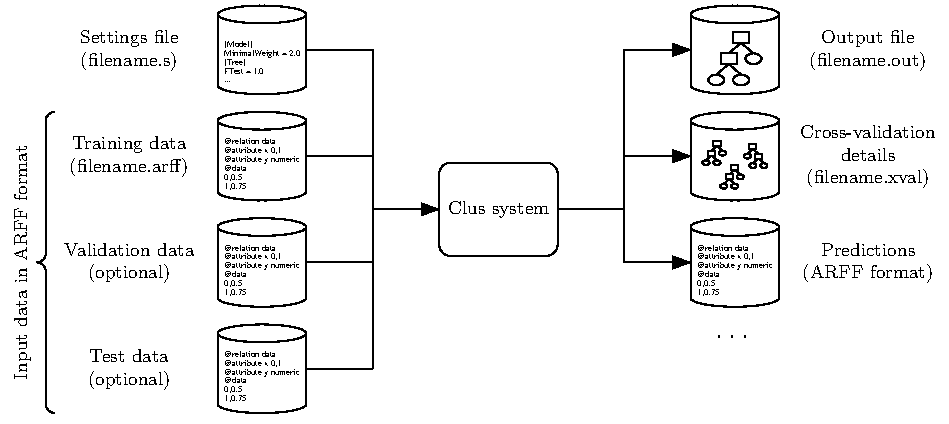
\includegraphics{fig/clusinout}
\end{figure}

Clus uses two input files, with the names {\tt {\em app}.s} and {\tt {\em app}.arff}, with {\em app} a name chosen by the user.  The {\tt {\em app}.s} contains the parameter settings for Clus.  The {\tt {\em app}.arff} file contains the data to be read.  The results of a Clus run are put in an output file {\tt {\em app}.out}.  In the following chapters we discuss the formats of these files.

\section{Command line parameters for Clus}

Clus accepts a number of command line parameters which affect its behavior.  An overview of these parameters and their meaning is given in Chapter~\ref{param:ch}.

\chapter{Learning algorithms}

\section{Tree learning}

\subsection{Top-down induction}

\subsection{Beam search}

\subsection{Constrained induction}

\subsection{Ensembles}

\section{Rule learning}

\subsection{Sequential covering algorithm}

\subsection{Rule ensembles}

\chapter{Case studies}

\section{Multi-target regression and classification}

\section{Hierarchical multi-label classification}

\section{Time series clustering}

\section{Clustering with instance level constraints}

\chapter{Input format}

Like many machine earning systems, Clus learns from tabular data.
These data are assumed to be in the ARFF format that is also used by the Weka data mining tool.  Full details on ARFF can be found elsewhere \cite{arff?}.
We here only give a minimal description.

In the data table, each row represents an instance, and each column represents an attribute of the instances.  Each attribute has a name and a domain (the domain is the set of values it can take).  In the ARFF format, the names and domains of the attributes are declared up front, before the data are given.

An ARFF file follows the following format:

\begin{tabbing}
{\tt \% all comment lines are optional, start with \%, and can occur }\\
{\tt \% anywhere in the file}\\
\\
{\tt @relation} name\\
\\
{\tt @attribute} name domain\\
{\tt @attribute} name domain\\
...\\
\\
{\tt @data} name domain\\
value$_1$, value$_2$, ..., value$_n$\\
value$_1$, value$_2$, ..., value$_n$\\
\end{tabbing}

The domain of an attribute can be one of:
\begin{tabbing}
\tt real\\
{\tt \{ } nomvalue$_1$, nomvalue$_2$, ..., nomvalue$_n$ {\tt \} }\\
{\tt hierarchical} hvalue$_1$, hvalue$_2$, ..., hvalue$_n$
\end{tabbing}

The first option, {\tt real}, indicates that the domain is the set of real numbers.

The second type of domain is called a discrete domain.  Discrete domains are defined by enumerating the values they contain.  These values are nominal.

The third type of domain is called ``hierarchical multi-label".  It implies two things: first, the attribute takes as value a {\em set} of values from the domain, rather than a single value; second, the domain has a hierarchical structure.  The elements of the domain are typically denoted $v_1/v_2/.../v_i$ with $i \leq d$ where $d$ is the depth of the hierarchy.  This type of domain is useful in the context of hierarchical multi-label classification.  

The values in a	 row occur in the same order as the attributes: the $i$'th value is assigned to the $i$'th attribute.  Values in the rows must be real values if the domain of the corresponding attribute is continuous, or a member of the specified set of values if the domain is discrete.  For hierarchical multi-label attributes, a set of values from the domain can be given; this set is written by listing its elements separated by \verb^@^.

Figure~\ref{arff:fig} shows an example of an ARFF file.  An example of a table containing hierarchical multi-label attributes is shown in Figure~\ref{arffhmc:fig}.

\begin{figure}
\hrule
\begin{verbatim}
@relation weather

@attribute outlook {sunny, overcast, rainy}
@attribute temperature real
@attribute humidity real
@attribute windy {TRUE, FALSE}
@attribute play {yes, no}

@data
sunny,85,85,FALSE,no
sunny,80,90,TRUE,no
overcast,83,86,FALSE,yes
rainy,70,96,FALSE,yes
rainy,68,80,FALSE,yes
rainy,65,70,TRUE,no
overcast,64,65,TRUE,yes
sunny,72,95,FALSE,no
sunny,69,70,FALSE,yes
rainy,75,80,FALSE,yes
sunny,75,70,TRUE,yes
overcast,72,90,TRUE,yes
overcast,81,75,FALSE,yes
rainy,71,91,TRUE,no
\end{verbatim}
\hrule
\caption{An example ARFF file.}
\label{arff:fig}
\end{figure}

%\section{Hierarchical multi-label attributes}

\begin{figure}
\hrule
\begin{verbatim}
@relation simple

@attribute A     {a,b}
@attribute B     {1,2}
@attribute class hierarchical rec/sport/swim,rec/sport/run,rec/auto

@data
a, 1, rec/sport/swim
a, 2, rec/sport/run
a, 2, rec/sport/run@rec/sport/swim
b, 1, rec/sport
b, 2, rec/auto
\end{verbatim}
\hrule
\caption{An ARFF file that includes an hierarchical multi-label attribute.}
\label{arffhmc:fig}
\end{figure}

\chapter{Settings file}

The algorithms included in the Clus system have a number of parameters that influence their behavior.  Most parameters have a default setting; the specification of a value for such parameters is optional.  For parameters that do not have a default setting or which should get another value than the default, a value must be specified in the settings file, {\tt {\em app}.s}.

The settings file is structured into sections.  Each parameter belongs to a particular section.  Including the section headers is optional, however; these sections are meant to help users structure the settings file but are not mandatory.

We here explain the most common settings.  Figure~\ref{settings:fig} shows how they might occur in a settings file.

{\bf * jans: the most important settings are already included in the list below, but it is probably useful to list and discuss for each of the common applications (single/multi target classification/regression, HMC, time series prediction, ...) the most appropriate settings. I should probably also extend the explanation for many of the settings.}

In the following, we use the convention that $n$ is an integer, $r$ is a real, $s$ is a string, $y$ is an element of \{ {\tt Yes}, {\tt No} \}, and $o$ is another type of value.  Strings are denoted without quotes.

\section{General}

\begin{itemize}
\item {\tt RandomSeed = $n$} : $n$ is used to initialize the random generator.
Some procedures used by Clus (e.g., creation of cross-validation folds) are randomized, and as a result, different runs of Clus on identical data may still yield different outputs.  When Clus is run on identical input data with the same {\tt RandomSeed} setting, it is guaranteed to yield the same results.
\end{itemize}

\section{Data}

\begin{itemize}
\item {\tt File = $s$} : $s$ is the name of the file that contains the training set.  The default value for $s$ is {\tt {\em app}.arff}.  Clus can read compressed ({\tt .arff.gz}) or uncompressed ({\tt .arff}) data files.
\item {\tt TestSet = $o$} : when $o$ is {\tt None}, no test set is used; if $o$ is a number between 0 and 1, Clus will use a proportion $o$ of the data file as a separate test set (used for evaluating the model but not for training); if $o$ is a valid file name containing a test set in ARFF format, Clus will evaluate the learned model on this test set.
\item {\tt PruneSet = $o$} : defines whether and how to use a pruning set; the meaning of $o$ is identical as in the {\tt TestSet} setting
\item {\tt XVal = $n$} : $n$ is the number of folds to be used in a cross-validation.  To perform cross-validation, Clus needs to be run with the {\tt -xval} option.
\end{itemize}

\section{Attributes}

\begin{itemize}
\item {\tt Target = $o$} : sets the index of the target attributes.  Attributes are numbered 1 through $n$.  $o$ is a comma-separated list of integers $i$ or intervals $i-j$; e.g., {\tt 5,7-9} indicates that attributes 5, 7, 8 and 9 are target values.  Run {\tt clus -info ...} to list all attributes.
{\bf * hb: klopt dit? originele doc suggereerde dat er maar 1 target kon zijn, maar dat is niet zo?}
\item {\tt Disable = $o$} : disables the listed attributes (they will not be used for prediction).  Attributes are numbered 1 through $n$.  $o$ is a comma-separated list of integers $i$ or intervals $i-j$; e.g., {\tt 5,7-9} indicates that attributes 5, 7, 8 and 9 are target values.  Run {\tt clus -info ...} to list all attributes.
\item {\tt Key = $o$} : with $o$ an attribute index, sets the key attribute; $o$ can be {\tt None}. 
   {\bf * hb: what is this useful for?}
\item {\tt Weight = $o$} : if $o$ = {\tt Normalize}, all numeric attributes are normalized.
   {\bf * hb: other options?}
\end{itemize}

\section{Model}

\begin{itemize}
\item {\tt MinimalWeight = $r$} : Clus only generates splits with at least $r$ instances in each subset.
\end{itemize}

\section{Tree}

\begin{itemize}
\item {\tt FTest = $r$} : sets the f-test stopping criterion for regression; a node will only be split if a statistical F-test indicates a significant (at level $r$) reduction of variance inside the subsets.
\item {\tt MaxDepth = $o$} : $o$ is a positive integer or {\tt Infinity}.  Clus will build trees with depth at  most $o$.
\item {\tt ConvertToRules = $o$} : $o$ is {\tt Yes} or {\tt No}.  If {\tt Yes},  Clus will convert the induced tree to a set of rules.
\end{itemize}

\section{Rules}


\section{Ensembles}

\section{Constraints}

\begin{itemize}
\item {\tt Syntactic = $o$} : sets the file with syntactic constraints (e.g., a partial tree) \cite{paper-on-constraints}
\item {\tt MaxSize = $o$} : sets the maximum size for Garofalakis pruning \cite{Garofalakis}; $o$ can be a positive integer or {\tt Infinity}
\item {\tt MaxError = $o$} : sets the maximum error for Garofalakis pruning; $o$ is a positive real or {\tt Infinity}
\end{itemize}

\section{Output}

\begin{itemize}
\item {\tt AllFoldModels = $y$} : if set to {\tt Yes}, Clus will output the model built in each fold of a cross-validation
\item {\tt AllFoldErrors = $y$} : if set to {\tt Yes}, Clus will output the test set error (and other evaluation measures) for each fold
\item {\tt TrainErrors = $y$} : if set to {\tt Yes}, Clus will output the training set error (and other evaluation measures)
\item {\tt UnknownFrequency = $y$} : if set to {\tt Yes}, Clus will show in each node of the tree the proportion of instances that had a missing value for the test in that node
\item {\tt BranchFrequency = $y$} : if set to {\tt Yes}, Clus will show in each node of the tree, for each possible outcome of the test in that node, the proportion of instances that had that outcome
\item {\tt WritePredictions = $o$} : {\bf * hb: weet niet wat de \{Train,Test\} verzameling hier betekent}
\end{itemize}

\section{Beam}

\begin{itemize}
\item {\tt SizePenalty = $o$} : sets the size penalty parameter used in the beam heuristic \cite{beam-paper}
\item {\tt BeamWidth = $n$} : sets the width of the beam used in the beam search performed by Clus \cite{beam-paper}
\item {\tt MaxSize = $o$} : sets the maximum size constraint \cite{beam-paper}; $o$ is a positive integer or {\tt Infinity}
\end{itemize}

\begin{figure}
\hrule
\begin{verbatim}
[General]
RandomSeed = 0              % seed of random generator

[Data]
File = iris.arff            % training data
TestSet = None              % data used for evaluation (file name / proportion)
PruneSet = None             % data used for tree pruning (file name / proportion)
XVal = 10                   % number of folds in cross-validation (clus -xval ...)

[Attributes]
Target = 5                  % index of target attributes
Disable = 4                 % Disables some attributes (e.g., "5,7-8")
Key = None                  % Sets the index of the key attribute
Weights = Normalize         % Normalize numeric attributes

[Model]
MinimalWeight = 2.0         % at least 2 examples in each subtree
         
[Tree]
FTest = 1.0                 % f-test stopping criterion for regression
MaxDepth = Infinity         % Stop building the tree at the given depth
ConvertToRules = No         % Convert the tree to a set of rules

[Constraints]
Syntactic = None            % file with syntactic constraints (a partial tree)
MaxSize = Infinity          % maximum size for Garofalakis pruning
MaxError = Infinity         % maximum error for Garofalakis pruning

[Output]
AllFoldModels = Yes         % Output model in each cross-validation fold
AllFoldErrors = No          % Output error measures for each fold
TrainErrors = Yes           % Output training error measures
UnknownFrequency = No       % proportion of missing values for each test
BranchFrequency = No        % proportion of instances for which test succeeds
WritePredictions = {Train,Test}    % write test set predictions to file

[Beam]
SizePenalty = 0.1           % size penalty parameter used in the beam heuristic
BeamWidth = 10              % beam width
MaxSize = Infinity          % Sets the maximum size constraint
\end{verbatim}
\hrule
\caption{An example settings file}
\label{settings:fig}
\end{figure}


\section{Hierarchical}

A number of settings are relevant only when using Clus for Hierarchical Multi-label Classification (HMC).  These go in the separate section ``Hierarchical''.  The most important ones are:

\begin{itemize}
\item {\tt Type = $o$} : $o$ is {\tt Tree} or {\tt DAG}, and indicates whether the class hierarchy is a tree or a directed acyclic graph \cite{hmc-paper}
\item {\tt WType = $o$} : defines how parents' class weights are aggregated in DAG-shaped hierarchies (\cite{Vens08:jrnl}, Section 4.1): possible values are {\tt ExpSumParentWeight}, {\tt ExpAvgParentWeight}, {\tt ExpMinParentWeight}, {\tt ExpMaxParentWeight}, and {\tt NoWeight}.  These define the weight of a class to be $w_0$ times the sum, average, minimum or maximum of the parent's weights, respectively, or to be 1.0 for all classes. 
\item {\tt WParam = $r$} : sets the parameter $w_0$ used in the formula for defining the class weights (\cite{Vens08:jrnl}, Section 4.1)
\item {\tt HSeparator = $o$} : $o$ is the separator used in the notation of values of the hierarchical domain (typically `/' or `.') 
\item {\tt EmptySetIndicator = $o$} : $o$ is the symbol used to indicate the empty set
\item {\tt OptimizeErrorMeasure = $o$} : Clus can automatically optimize the {\tt FTest} setting; $o$ indicates what criterion should be maximized for this (\cite{Vens08:jrnl}, Section 5.2).  Possible values for $o$ are:
  \begin{itemize}
   \item {\tt AverageAUROC}: average of the areas under the class-wise ROC curves
   \item {\tt AverageAUPRC}: average of the areas under the class-wise precision-recall curves
   \item {\tt WeightedAverageAUPRC}: similar to AverageAUPRC, but each class's contribution is                         weighted by its relative frequency
   \item {\tt PooledAUPRC}: area under the average (or pooled) precision-recall curve
  \end{itemize}
\item {\tt ClassificationThreshold = $o$} : The original tree constructed by Clus contains a vector of predicted probabilities (one for each class) in each leaf. Such a probabilistic prediction can be converted into a set of labels by applying a threshold $t$: all labels that are predicted with probability $> t$ are in the predicted set.  $o$ can be a set of thresholds, e.g., \{0.5, 0.75, 0.80, 0.90, 0.95\}. Clus will output for each value in the set a tree in which the predicted label sets are constructed with this particular threshold. So, in the example, the output file will contain 5 trees corresponding to the thresholds 0.5, 0.75, 0.80, 0.90 and 0.95.
{\bf * hb: is the set of thresholds indeed written as a set, i.e. between curly braces?  And is it really $>t$, or $\geq t$?}
\item {\tt RecallValues = $o$} : $o$ is a list of recall values. For each value, Clus will output the average of the precisions over all class-wise precision-recall curves that correspond to the particular recall value in the output file.
{\bf * hb: "list": how is it denoted?}
\item {\tt EvalClasses = $o$} : If $o$ is {\tt None}, Clus computes average error measures across all classes in the class  hierarchy. If $o$ is a list of classes, then the error measures are only computed with regard to the classes in this list.
\end{itemize}

Figure~\ref{settings-hmc:fig} summarizes these briefly.

\begin{figure}
\hrule
\begin{verbatim}
[Hierarchical]
Type = Tree                         % Tree or DAG hierarchy?
WType = ExpAvgParentWeight          % aggregation of class weights
WParam = 0.75                       % parameter w_0
HSeparator = /                      % separator used in class names
EmptySetIndicator = n               % symbol for empty set
OptimizeErrorMeasure = PooledAUPRC  % FTest optimization strategy
ClassificationThreshold = None      % threshold for "positive"
RecallValues = None                 % where to report precision
EvalClasses = None                  % classes to evaluate
\end{verbatim}
\hrule
\caption{Settings specific for hierarchical multi-label classification}
\label{settings-hmc:fig}
\end{figure}

\chapter{Output file}

When Clus is finished, it writes the results of the run into an output file with the name
{\tt {\em app}.out}.  An example of such an output file is shown in Figures \ref{output1:fig} to \ref{output4:fig}.

\begin{figure}
\hrule
\begin{verbatim}
Clus run iris
*************

Date: 11/20/09 3:39 PM
File: iris.out
Attributes: 5 (input: 4, output: 1)
Missing values: No

[General]
Verbose = 1
Compatibility = Latest
RandomSeed = 0
ResourceInfoLoaded = No

[Data]
File = iris.arff
TestSet = None
PruneSet = None
XVal = 10
RemoveMissingTarget = No
NormalizeData = None

[Attributes]
Target = 5
Clustering = 5
Descriptive = 1-4
Key = None
Disable = None
Weights = Normalize
ClusteringWeights = 1.0
ReduceMemoryNominalAttrs = No

[Constraints]
Syntactic = None
MaxSize = Infinity
MaxError = 0.0
\end{verbatim}
\hrule
\caption{Example output file (part 1, settings).}
\label{output1:fig}
\end{figure}

\begin{figure}
\hrule
\small
\begin{verbatim}
[Output]
ShowModels = {Default, Pruned, Others}
TrainErrors = Yes
ValidErrors = Yes
AllFoldModels = Yes
AllFoldErrors = No
AllFoldDatasets = No
WriteErrorFile = No
UnknownFrequency = No
BranchFrequency = No
ShowInfo = {Count}
PrintModelAndExamples = No
WritePredictions = {None}
ModelIDFiles = No
OutputPythonModel = No
OutputDatabaseQueries = No
WriteCurves = No

[Nominal]
MEstimate = 1.0

[Model]
MinimalWeight = 2.0
MinimalNumberExamples = 0
ParamTuneNumberFolds = 10
ClassWeights = 0.0
NominalSubsetTests = Yes

[Tree]
Heuristic = Gain
MaxDepth = Infinity
BinarySplit = Yes
PruningMethod = C4.5
MSENominal = No
ConvertToRules = No
AlternativeSplits = No
Optimize = {}

[SIT]
Main_target = Default
Recursive = No
Search = OneTarget
Learner = ClusLearner
Error = MSE
\end{verbatim}
\hrule
\caption{Example output file (part 2, settings (ctd.)).}
\label{output2:fig}
\end{figure}

\begin{figure}
\hrule
\footnotesize
\begin{verbatim}
Run: 01
*******

Statistics
----------
FTValue (FTest): 1.0
Induction Time: 0.019 sec
Pruning Time: 0.003 sec
Model information
     Default: Nodes = 1 (Leaves: 1)
     Original: Nodes = 9 (Leaves: 5)
     Pruned: Nodes = 9 (Leaves: 5)

Training error
--------------
Number of examples: 150
Classification Error
   Default: 
   Attribute: class
           REAL\PRED | Iris-setosa | Iris-versicolor | Iris-virginica |
     ----------------------------------------------------------------------
         Iris-setosa |          50 |               0 |              0 |  50
     Iris-versicolor |          50 |               0 |              0 |  50
      Iris-virginica |          50 |               0 |              0 |  50
     ----------------------------------------------------------------------
                     |         150 |               0 |              0 | 150
     Accuracy: 0.333333
     Cramer's coefficient: 0

   Original: 
   Attribute: class
           REAL\PRED | Iris-setosa | Iris-versicolor | Iris-virginica |
     ----------------------------------------------------------------------
         Iris-setosa |          50 |               0 |              0 |  50
     Iris-versicolor |           0 |              49 |              1 |  50
      Iris-virginica |           0 |               2 |             48 |  50
     ----------------------------------------------------------------------
                     |          50 |              51 |             49 | 150
     Accuracy: 0.98
     Cramer's coefficient: 0.970555

   Pruned: 
   Attribute: class
           REAL\PRED | Iris-setosa | Iris-versicolor | Iris-virginica |
     ----------------------------------------------------------------------
         Iris-setosa |          50 |               0 |              0 |  50
     Iris-versicolor |           0 |              49 |              1 |  50
      Iris-virginica |           0 |               2 |             48 |  50
     ----------------------------------------------------------------------
                     |          50 |              51 |             49 | 150
     Accuracy: 0.98
     Cramer's coefficient: 0.970555

Weighted mean squared error (MSE) for Nominal Attributes (Weights [1.5])
   Default        : [1]
   Original       : [0.0525]
   Pruned         : [0.0525]
\end{verbatim}
\hrule
\caption{Example output file (part 3, statistics).}
\label{output3:fig}
\end{figure}

\begin{figure}
\hrule
\begin{verbatim}
Default Model
*************

[Iris-setosa] [50.0]: 150

Original Model
**************

petallength > 1.9
+--yes: petalwidth > 1.7
|       +--yes: [Iris-virginica] [45.0]: 46
|       +--no:  petallength > 4.9
|               +--yes: petalwidth > 1.5
|               |       +--yes: [Iris-versicolor] [2.0]: 3
|               |       +--no:  [Iris-virginica] [3.0]: 3
|               +--no:  [Iris-versicolor] [47.0]: 48
+--no:  [Iris-setosa] [50.0]: 50

Pruned Model
************

petallength > 1.9
+--yes: petalwidth > 1.7
|       +--yes: [Iris-virginica] [45.0]: 46
|       +--no:  petallength > 4.9
|               +--yes: petalwidth > 1.5
|               |       +--yes: [Iris-versicolor] [2.0]: 3
|               |       +--no:  [Iris-virginica] [3.0]: 3
|               +--no:  [Iris-versicolor] [47.0]: 48
+--no:  [Iris-setosa] [50.0]: 50
\end{verbatim}
\hrule
\caption{Example output file (part 4, learned models).}
\label{output4:fig}
\end{figure}

\section{Used settings}

The first part of {\tt {\em app}.out} (shown in Figures \ref{output1:fig} and \ref{output2:fig}) contains the values of the settings that were used for this run of Clus, in the format used by the settings file.  This part can be copied and pasted to {\tt {\em app}.s} and modified for subsequent runs.

\section{Evaluation statistics}

The next part contains statistics about the results of this Clus run.

Summary statistics about the running time of Clus and about the size of the resulting models are given.  Next, information on the models' predictive performance on the training set (``training set error") is given, as well as an estimate of its predictive performance on unseen examples (``test set error"), when available (this is the case if a cross-validation or an evaluation on a separate test set was performed).  

Typically three models are reported: a ``default'' model consisting of a tree of size zero, which can be used as a reference point (for instance, its predictive accuracy equals that obtained by always predicting the majority class); an unpruned (``original") tree, and a pruned tree.

For classification trees the information given for each model by default includes a contingency table, and (computed from that) the accuracy and Cramer's correlation coefficient.

{\bf * jans: For a binary attribute, the ``weighted MSE for nominal attributes" is the MSE of the 0/1 representation of the attribute. Similarly, a non-binary attribute $A$ with $m$ values can be represented by $m$ binary attributes such that the $i$-th binary attribute is equal to 1 if and only if $A$ takes the $i$-th value from its domain. In this case, the error measure is the average MSE across these $m$ binary attributes. This error measure is precisely the error measure that is locally optimized by the Gini index heuristic.

Merk op: Deze MSE voor nominale attributen was maar iets dat ik heb toegevoegd voor een bepaald experiment. Misschien kan ik het beter terug weghalen want het is nogal complex.}

For regression trees, this information includes the mean absolute error (MAE), mean squared error (MSE), root mean squared error (RMSE), weighted RMSE, the Pearson correlation coefficient $r$ and it square.  In the weighted RMSE, the weight of a given attribute $A$ is its normalization weight, which is $\frac{1}{\sqrt{\mathrm{Var}(A)}}$, with $\mathrm{Var}(A)$ equal to $A$'s variance in the input data. 


\section{The models}

The output file contains the learned models, represented as decision trees.  The level of detail in which the models are shown is influenced by certain settings.


\chapter{Command line parameters}
\label{param:ch}

Clus is run from the command line.  It takes a number of command line parameters that affect its behavior.

\begin{itemize}
\item {\tt -xval} : in addition to learning a single model from the whole input dataset, perform a cross-validation.  The xval setting determines the number of folds; the random\_seed setting initializes the random generator that determines the folds.
\item {\tt -info} : gives information and summary statistics about the dataset.
\item ...
\end{itemize}

\chapter{Developer Documentation}

\section{Compiling Clus}

Note: The Clus download comes with a pre-compiled version of Clus 
stored in the file Clus.jar. So, if you just want to run Clus as it is on a 
data set, then you do not need to compile Clus. You can run it using the
above instructions. On the other hand, if you wish to modify the source 
code of Clus, or if you are using the CVS version, then you will need to 
compile the source code of Clus. This can be done using the commands
below or using the Eclipse IDE as pointed out in the next section.

(Windows)

\begin{small}
\begin{verbatim}
cd C:\Clus\src
javac -d "bin" -cp ".;jars\commons-math-1.0.jar;jars\jgap.jar" clus/Clus.java
\end{verbatim}
\end{small}

(Unix)

\begin{small}
\begin{verbatim}
cd /home/john/Clus
javac -d "bin" -cp ".:jars/commons-math-1.0.jar:jars/jgap.jar" clus/Clus.java
\end{verbatim}
\end{small}

This will compile Clus and write the resulting .class files (Java executable 
byte code) to the "bin" subdirectory.

Alternatively, use the "./compile.sh" script provided in the Clus main directory.

\section{Compiling Clus with Eclipse}

In Eclipse, create a new project for Clus as follows:

\begin{itemize}
\item Choose \verb^File | New | Project^.
\item Select "Java Project" in the dialog box.
\item In the "New Java Project" dialog box:
 \begin{itemize}
 \item Enter "Clus" in the field "Project Name".
 \item Choose "Create project from existing source" and browse to the location where 
      you unzipped Clus. E.g., \verb^/home/john/Clus^ or \verb^C:\Clus^.
 \item Click "Next".
 \item Select the "Source" tab of the build settings dialog box.
     Change "Default output folder" (where the class files are generated) to: "Clus/bin".
 \item Select the "Libraries" tab of the build settings dialog box.
     Click "Add external jars" and add in this way these three jars:\\
        Clus/jars/commons-math-1.0.jar\\
        Clus/jars/jgap.jar\\
        Clus/jars/weka.jar
 \item Click "Finish".
 \end{itemize}
\item Select the "Navigator" view (Choose Window | Show View | Navigator)
 \begin{itemize}
   \item  Right click the "Clus" project in this view.
   \item  Select "Properties" from the context menu.
   \item  Select the "Java Compiler" tab.
   \item  Set the "Java Compliance Level" to 5.0.
 \end{itemize}
\end{itemize}
Now Clus should be automatically compiled by Eclipse.
To run Clus from Eclipse:
 \begin{itemize}
   \item Set as main class "clus.Clus".
   \item Set as arguments the name of your settings file (appfile.s).
   \item Set as working directory, the directory on the file system where your data set is located.
\end{itemize}

\section{Running Clus after compiling the source code}

These instructions are for running Clus after you compiled its source code (using the instructions "Compiling Clus" or "Compiling Clus with Eclipse"). To run the pre-compiled version that is available in the file "Clus.jar", see above.

(Windows)
\begin{small}
\begin{verbatim}
cd path\to\appfile.s
java -cp "C:\Clus\bin;C:\Clus\jars\commons-math-1.0.jar;C:\Clus\jars\jgap.jar" 
  clus.Clus appfile.s
\end{verbatim}
\end{small}

(Unix)

\begin{small}
\begin{verbatim}
cd path/to/appfile.s
java -cp "$HOME/Clus/bin:$HOME/Clus/jars/commons-math-1.0.jar:$HOME/Clus/jars/jgap.jar" 
  clus.Clus appfile.s
\end{verbatim}
\end{small}

Alternatively, use the "./clus.sh" script provided in the Clus main directory after adjusting the line that defines CLUS\_DIR at the top of the script.

\bibliographystyle{plain}
\bibliography{.mlbib}

\end{document}
